% !TeX program = xelatex
\documentclass[12pt,a4paper]{article}
\usepackage{fontspec}
\setmainfont{Times New Roman}
\setsansfont{Arial}
\setmonofont{Courier New}
\usepackage[english,russian]{babel}
\usepackage{amsmath,amssymb}
\usepackage[margin=22mm]{geometry}
\usepackage{graphicx,float}
\usepackage[unicode,hidelinks]{hyperref}
\setlength{\emergencystretch}{3em}
\interfootnotelinepenalty=10000
\newcommand{\topic}[1]{\par\medskip\noindent\textbf{#1}\par\nobreak\smallskip}
\renewcommand{\thefootnote}{\arabic{footnote})}
\DeclareMathOperator{\grad}{grad}
\DeclareMathOperator{\Div}{div}
\title{Вопрос 4. Фильтрация несжимаемой жидкости. Одномерные течения и формула Дюпюи}
\author{Н. Е. Леонтьев\\\large Основы теории фильтрации}
\date{Учебное пособие. 2-е издание. Москва: МАКС Пресс, 2017\\Глава II, § 7. Печатные страницы 38--43}
\begin{document}
\maketitle
\noindent\textit{Полный перенос § 7, до заголовка § 8 на странице 43. Номера страниц PDF совпадают с печатными. Размещение материала перевёрстано.}
% Источник: Leontiev-2017.pdf; печатная страница: 38; страница файла: 38
\section*{Глава II. Фильтрация несжимаемой жидкости в недеформируемой пористой среде}
\label{q4:chapter-ii}
\subsection*{§ 7. Замкнутая система уравнений и простейшие задачи}
\label{q4:sec-7}
\topic{Замкнутая система уравнений}
\setcounter{footnote}{0}
Полная система уравнений, описывающих \textit{стационарную} фильтрацию однородной несжимаемой жидкости в однородной изотропной пористой среде, состоит из уравнения неразрывности и закона фильтрации:
\begin{equation}
\Div\boldsymbol{u}=0,\qquad 0=-\grad p+\rho\boldsymbol{F}-\frac{\mu}{k}\boldsymbol{u}.
\tag{7.1}\label{q4:eq-7-1}
\end{equation}
Это система четырех скалярных уравнений относительно четырех неизвестных (давления $p$ и трех компонент скорости фильтрации $\boldsymbol{u}$). Если рассматривается фильтрация в однородном поле тяжести, то закон Дарси удобно использовать в форме (3.6), инвариантная запись которой имеет вид
\begin{equation}
\boldsymbol{u}=-C\grad H,\qquad C=\frac{k\rho g}{\mu},\qquad H=\frac{p}{\rho g}-\boldsymbol{r}\cdot\frac{\boldsymbol{g}}{g}.
\tag{7.2}\label{q4:eq-7-2}
\end{equation}
После подстановки \eqref{q4:eq-7-2} в уравнение неразрывности получается уравнение Лапласа относительно напора $H$\footnote{Или, что эквивалентно, уравнение Лапласа относительно давления: $\triangle p=0$.}:
\begin{equation}
\triangle H=\frac{\partial^2H}{\partial x^2}+\frac{\partial^2H}{\partial y^2}+\frac{\partial^2H}{\partial z^2}=0,
\tag{7.3}\label{q4:eq-7-3}
\end{equation}
к решению которого при заданных граничных условиях и сводится задача. После нахождения $H(x,y,z)$ поле скоростей находится с помощью закона Дарси \eqref{q4:eq-7-2}.

Система \eqref{q4:eq-7-1} годится и для описания \textit{нестационарной} фильтрации. При этом зависимость от времени может учитываться как через параметры, входящие в закон фильтрации (скажем, внешние массовые силы могут зависеть от времени, например при исследовании пористого образца на центрифуге), так и через граничные условия (примеры: повышение давления на дне при поднятии уровня воды в реке во время половодья; растекание «бугра» грунтовых вод, образовавшегося после дождя, когда нестационарность проявляется в изменении формы свободной поверхности).

% Источник: Leontiev-2017.pdf; печатная страница: 39; страница файла: 39
Фильтрация в \textit{анизотропной} среде с постоянным тензором проницаемости в ряде случаев также может быть сведена к решению уравнения \eqref{q4:eq-7-3} за счет выбора прямоугольной системы координат, в которой матрица $(k_{ij})$ диагонализируется, и изменения линейных масштабов по осям координат. При этом граничные условия также преобразуются соответствующим образом.

Приведем несколько простейших задач, решающихся с помощью приведенной модели.

\topic{Опыт Дарси}
\setcounter{footnote}{0}
Для экспериментального определения проницаемости пористой среды можно использовать установку (рис.~\ref{q4:fig-11}), в которой жидкость под действием силы тяжести просачивается через находящийся в вертикальном канале слой пористого материала\footnote{Классические опыты Дарси проводились на установке именно с такой схемой.}. Пористый образец удерживается снизу сеткой, которая не мешает жидкости высачиваться на нижней поверхности образца и стекать в емкость под установкой.

\setcounter{figure}{10}
\begin{figure}[H]
\centering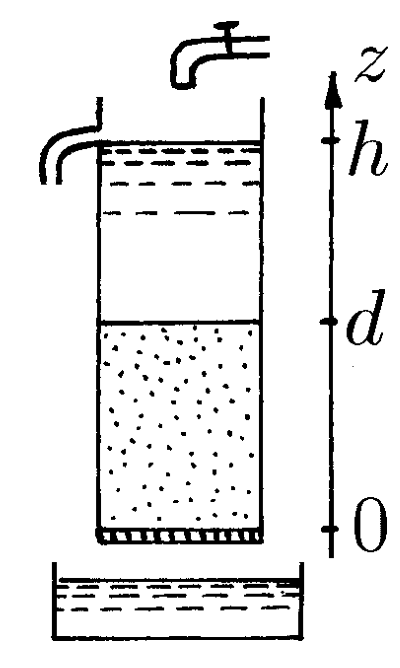
\includegraphics[width=.22\linewidth]{figures/figure-11.png}
\caption{}\label{q4:fig-11}
\end{figure}
Для простоты будем считать величину внешнего атмосферного давления равной нулю, поскольку добавление произвольной константы к напору не меняет поля скорости фильтрации. Пусть высота пористого образца равна $d$, а свободный уровень жидкости в верхней части установки поддерживается на постоянной высоте $h$ относительно нижней поверхности образца (жидкость все время доливается из крана, находящегося над установкой, а в боковой стенке установки имеется слив, не позволяющий уровню жидкости подняться выше $h$).

Выбрав начало координат в плоскости нижнего основания образца и направив ось $z$ вертикально вверх, получим задачу о нахождении решения уравнения Лапласа \eqref{q4:eq-7-3} в области, занятой пористым образцом, со следующими граничными условиями:

условие непротекания на непроницаемых боковых стенках
\[
\grad H\cdot\boldsymbol{n}=\frac{\partial H}{\partial n}=0,
\]
постоянство напора на нижней поверхности (поверхности
% Источник: Leontiev-2017.pdf; печатная страница: 40; страница файла: 40
высачивания)
\[
\left.H\right|_{z=0}=\left.\left(\frac{p}{\rho g}+z\right)\right|_{z=0}=0,
\]
постоянство напора на верхней поверхности (границе жидкости и пористой среды)
\[
\left.H\right|_{z=d}=\left.\left(\frac{p}{\rho g}+z\right)\right|_{z=d}=\frac{\rho g(h-d)}{\rho g}+d=h.
\]
Решением этой краевой задачи является линейная функция $H(z)=hz/d$, а распределения скорости фильтрации и давления имеют вид
\[
\boldsymbol{u}=-C\grad H=(0;0;-Ch/d),\quad p(z)=\frac{\rho g(h-d)}{d}\,z.
\]
Таким образом, в этой задаче скорость фильтрации постоянна во всех точках пористого образца и направлена вертикально вниз, а давление жидкости изменяется вдоль образца по линейному закону.

При $h\to d$ из этого решения следует \textit{физический смысл} коэффициента фильтрации: если толщина слоя жидкости мала по сравнению с высотой образца и фильтрация происходит в основном за счет действия силы тяжести, то величина скорости фильтрации приближенно равна $C$\setcounter{footnote}{0}\footnote{Пример из повседневной жизни: при просачивании в сухой грунт воды из лужи под ней расширяется область смоченной пористой среды, ниже которой находится сухой грунт с атмосферным давлением в порах. Через некоторое время вертикальные размеры смоченной области становятся много больше глубины лужи и скорость фильтрации из нее, если воспользоваться приведенным решением для грубых прикидочных оценок, будет порядка коэффициента фильтрации грунта.}.

\topic{Точечный источник в пористой среде}
Предположим, что в некоторую точку пористого пласта, находящуюся вдали от границ пласта, пробурена скважина, через конец которой закачивается (или выкачивается) несжимаемая жидкость с объемным расходом $Q$ (рис.~\ref{q4:fig-12}). На расстояниях, много больших толщины скважины, возникающее течение можно рассматривать как сферически симметричное течение от точечного источника. Распределение напора $H(r)$, где $r$ --- расстояние
% Источник: Leontiev-2017.pdf; печатная страница: 41; страница файла: 41
до источника, определяется из уравнения Лапласа в сферических координатах
\[
\frac{1}{r^2}\frac{d}{dr}\left(r^2\frac{dH}{dr}\right)=0
\]
и имеет вид $H(r)=A/r+\mathrm{const}$, где постоянная $A$ определяется расходом $Q$, одинаковым для любой сферы радиуса $R$:
\[
Q=4\pi R^2\left.u\right|_{r=R}=\left.4\pi R^2\left(-C\frac{dH}{dr}\right)\right|_{r=R}=4\pi A,
\]
% В оригинале правая часть напечатана как 4πA, без множителя C. Сохранено дословно; не исправлять молча.
что дает
\begin{equation}
H(r)=\frac{Q}{4\pi C}\frac{1}{r}+\mathrm{const}.
\tag{7.4}\label{q4:eq-7-4}
\end{equation}
\begin{figure}[H]
\centering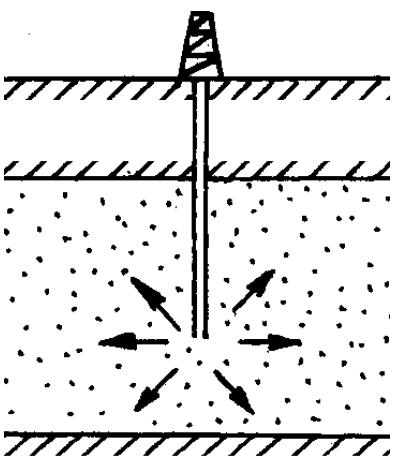
\includegraphics[width=.23\linewidth]{figures/figure-12.png}
\caption{}\label{q4:fig-12}
\end{figure}
Значение $Q>0$ соответствует источнику (закачке жидкости в пласт), значение $Q<0$ --- стоку (выкачиванию жидкости из пласта). При приближении к источнику (при $r\to0$) скорость фильтрации стремится к бесконечности, поэтому при практическом применении эту формулу нужно использовать начиная с расстояний, соизмеримых с реальным размером источника (например, толщиной скважины).

С помощью \eqref{q4:eq-7-4} легко найти выражение расхода $Q$ через значения напора $H(r_1)$ и $H(r_2)$ в двух точках пласта на расстояниях $r_1$ и $r_2$ от источника:
\[
Q=4\pi C\frac{H(r_2)-H(r_1)}{\dfrac{1}{r_2}-\dfrac{1}{r_1}},
\]
которое удобно использовать на практике.

Обратим внимание, что в окрестности скважины значения скорости фильтрации могут быть настолько больш\'ими, что вместо закона Дарси нужно использовать, например, двучленный закон фильтрации (4.3), который в терминах напора в сферически симметричном случае имеет вид
\[
-C\frac{dH}{dr}=u+\frac{\beta\rho\sqrt{k}}{\mu}\,u^2.
\]
% Источник: Leontiev-2017.pdf; печатная страница: 42; страница файла: 42
Зависимость $H(r)$ в этом случае легко находится после подстановки в последнее уравнение распределения скорости фильтрации
\[
u(r)=\frac{Q}{4\pi r^2}.
\]

\topic{Скважина, вскрывающая тонкий пласт}
Находящиеся в недрах земли жидкие и газообразные полезные ископаемые как правило сосредоточены в тонких пластах, окруженных сверху и снизу менее проницаемыми породами. Например, толщины нефтяных пластов, залегающих на разных глубинах, имеют обычно порядок метров или десятков метров, в то время как их горизонтальная протяженность может составлять километры. Поэтому течение вокруг работающей скважины, целиком вскрывающей тонкий однородный продуктивный пласт (рис.~\ref{q4:fig-13}), можно приближенно рассматривать как одномерное осесимметричное (при условии, конечно, что скважина находится на большом расстоянии от других скважин и контура пласта).

\begin{figure}[H]
\centering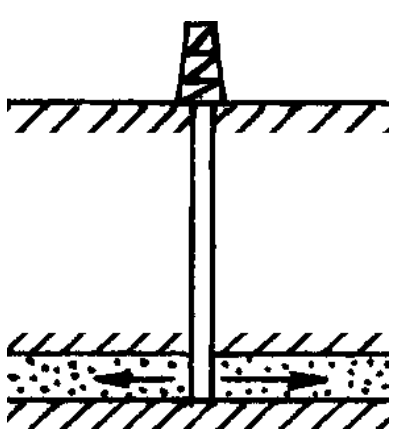
\includegraphics[width=.22\linewidth]{figures/figure-13.png}
\caption{}\label{q4:fig-13}
\end{figure}
В случае работы скважины с постоянным погонным (на единицу толщины пласта) расходом $Q$ распределение напора находится из уравнения Лапласа в цилиндрических координатах
\[
\frac{1}{r}\frac{d}{dr}\left(r\frac{dH}{dr}\right)=0
\]
с условием
\[
Q=2\pi R\left.u\right|_{r=R}=-\left.2\pi RC\frac{dH}{dr}\right|_{r=R}
\]
при любом $r=R$, что дает
\[
H(r)=-\frac{Q}{2\pi C}\ln\frac{r}{r_0},\qquad r_0=\mathrm{const}.
\]
Как и в случае точечного источника, расход выражается через значения напора в двух точках на разных расстояниях от скважины:
\begin{equation}
Q=-2\pi C\frac{H(r_2)-H(r_1)}{\ln(r_2/r_1)}.
\tag{7.5}\label{q4:eq-7-5}
\end{equation}
% Источник: Leontiev-2017.pdf; печатная страница: 43; страница файла: 43
Это соотношение называется \textit{формулой Дюпю\'и} (J.Dupuit) для напорного притока к совершенной скважине\setcounter{footnote}{0}\footnote{Другая формула, носящая имя этого ученого, встретится в § 9.}.

Поясним название этой формулы. \textit{Безнапорной фильтрацией} называется фильтрация с образованием свободной поверхности (поверхности депрессии), в противном случае говорят о \textit{напорной фильтрации}.

Скважина называется \textit{совершенной}, если она целиком вскрывает пласт и флюид может перетекать в скважину (из скважины) через всю ее боковую поверхность, находящуюся в пласте. Если же скважина проникает в пласт не полностью либо не вся ее боковая поверхность, находящаяся в пласте, является проницаемой, то она называется \textit{несовершенной}. Несовершенство скважины обычно делает течение в непосредственной близости от нее неодномерным.

Обратим внимание на то, что в приведенном решении напор (а следовательно, давление) обращается в бесконечность не только в окрестности скважины, как это было в задаче о точечном источнике, но и на бесконечности, что, однако, не мешает практическому применению решения к реальным геологическим объектам с конечными размерами.
% Конец § 7. Далее на странице 43 начинается § 8 «Применение методов теории функций комплексного переменного для решения плоских фильтрационных задач».

\end{document}
